\section{Team Work}

\begin{itemize}
  \item Paul Wang: Verilog Implementation.
  \item Danny Wang: Report.
\end{itemize}

\section{Cache Controller}

The cache controller is the most important part of this project. The following figure is the FSM of the cache controller.

\begin{figure}[h!]
  \centering
  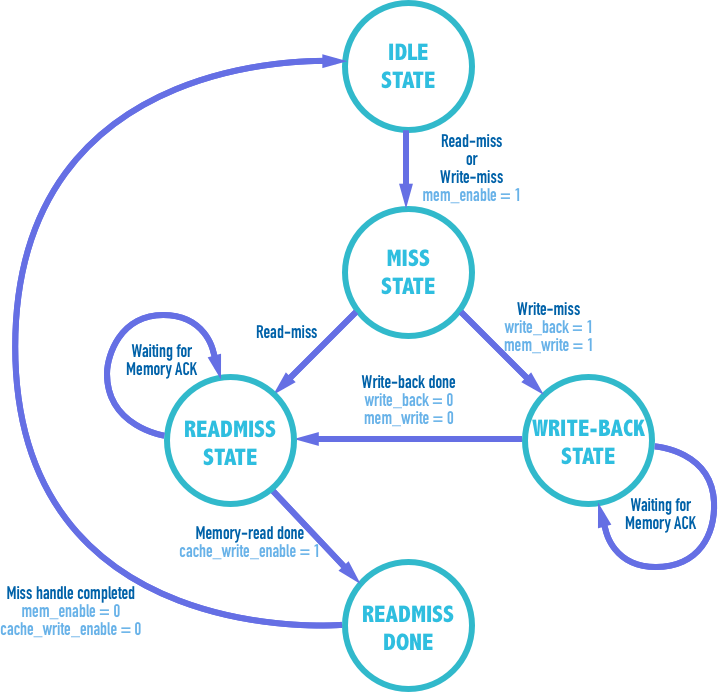
\includegraphics[width=.8\textwidth]{state.png}
\end{figure}

There are five states in the FSM, controlling 4 control signals (\texttt{write\_back} and \texttt{mem\_write} are actually identicali in this case). The functions of these signals are listed below:

\begin{enumerate}
  \item \texttt{mem\_enable}: controls the link between cache controller and memory.
  \item \texttt{write\_back}(\texttt{mem\_write}): signals memory that a write-back is required.
  \item \texttt{cache\_write\_enable}: controls the link between cache controller and cache sram.
\end{enumerate}

The FSM is in the Idle-State most of the time. It starts working only when either read-miss or write-miss occurs. Then if the block to be replaced has its dirty bit set, the controller signals memory to write the block back to memory. After write-back is completed, the new block is then loaded from memory. And we can guarantee a hit for the current instruction. One thing worth noting is that, we have to send a stall signal to the entire pipeline when we are waiting for memory access in order to ensure the correctness of the pipeline execution.

Other important control signals can be derived by inputs and the three control signals listed above, some are listed below (others can be found in the source code.)

\begin{lstlisting}
assign  p1_req     = p1_MemRead_i | p1_MemWrite_i;
assign  p1_stall_o = ~hit & p1_req;

// SRAM interface
assign  cache_sram_write  = cache_we | write_hit;
assign  cache_sram_tag    = {1'b1, cache_dirty, p1_tag};
assign  cache_sram_data   = (hit) ? w_hit_data : mem_data_i;

// memory interface
assign  mem_addr_o    = (write_back) ?
              {sram_tag, p1_index, 5'b0} : {p1_tag, p1_index, 5'b0};
assign  write_hit     = hit & p1_MemWrite_i;
assign  cache_dirty   = write_hit;

// tag comparator
assign  hit           = sram_valid && (sram_tag == p1_tag);
assign  r_hit_data    = (hit) ? sram_cache_data : mem_data_i;

// read data :  256-bit to 32-bit
always@(p1_offset or r_hit_data) begin
  case (p1_offset[4:2])
    3'd0: p1_data <= r_hit_data[31:0];
    ... (7 other cases)
  endcase
end

// write data :  32-bit to 256-bit
always@(p1_offset or r_hit_data or p1_data_i) begin
  w_hit_data[31:0]    = (p1_offset[4:2] == 3'd0) ?
                        p1_data_i : r_hit_data[31:0];
  ... (7 other cases)
end
\end{lstlisting}

\section{Problems \& Solutions}
No significant problems occured throughout this project. However, one thing that separates this project from project 1 is that we've isolated data memory from the CPU, which is a big step closer to the reality. And through this process, we get to think of the possible hardware interface between CPU and memory as well as the data transfer protocols that are involved.
